\documentclass[10.5pt]{article}
\usepackage[a4paper,margin=2.1cm]{geometry}
\usepackage{amsmath,amssymb}
\usepackage{booktabs}
\usepackage{graphicx}
\usepackage[hidelinks]{hyperref}
\usepackage{enumitem}
\usepackage{caption}
\usepackage{float}
\setlist{itemsep=1pt,topsep=2pt}
\captionsetup{font=small,labelfont=bf}
\newcommand{\code}[1]{\texttt{#1}}
\emergencystretch=3em
\author{Phung Gia Huy}
\date{November 2026}

\hypersetup{pdftitle={GStar Assignment 2, Problem 2: reasoning about poker with GRPO},pdfauthor={Phung Gia Huy}}
\title{\textbf{GStar Assignment 2 -- Problem 2 (extra credit)}\\[2pt]\large Teaching a small LLM to reason about poker with GRPO}

\begin{document}
\maketitle
\vspace{-10pt}
\begin{center}\small
Code: \code{problem2/} in the submission and at \url{https://github.com/huypg-zenai/GStar-Assignment-2-GRPO}
\end{center}

\section{What we chose to explore}
Countdown has one right answer per prompt. Many real decisions do not: the best action depends on hidden information and
on what other agents do. We chose the \emph{adaptation} direction, moving the Problem 1 pipeline to a game with hidden
information, and asked:

\begin{center}
\emph{Can GRPO teach Qwen3-1.7B to reason in such a setting, and does the reward design matter when feedback is noisy?}
\end{center}

\paragraph{The game: Leduc Hold'em.} A small poker game used in game-theory research:
\begin{itemize}
\item a 6-card deck (J J Q Q K K), one private card per player, and one public card revealed before round 2;
\item two betting rounds;
\item a pair (private card matches the public card) wins; otherwise the higher card wins.
\end{itemize}
It keeps the essence of poker (hidden information, bluffing, pot odds), yet has only 288 decision points. That makes two
things possible:
\begin{itemize}
\item solving it exactly with CFR+, which gives a perfect grader for every decision;
\item computing the \textbf{exploitability} of any strategy: the chips per hand a perfect adversary wins against it, with
  0 meaning unbeatable (equilibrium).
\end{itemize}
Our game engine matches OpenSpiel's \code{leduc\_poker} to 6 decimals.

\section{Approach}
\paragraph{Formulation.} Only the task changes; the GRPO code, GPUs and hyper-parameters are those of Problem 1
($L_{512}$, 80 steps).
\begin{itemize}
\item \textbf{Prompt:} one decision, described in plain English: the rules, the player's card, the public card if
  revealed, the betting so far, the pot, and the legal actions.
\item \textbf{Answer:} brief reasoning, then one action word in \code{<answer>} tags (for example
  \code{<answer>call</answer>}).
\end{itemize}

\paragraph{Training data.}
\begin{itemize}
\item Situations are generated from the game, so there is no dataset to download.
\item They are sampled half from equilibrium self-play (how often they arise in real play) and half uniformly at random
  (for coverage of rare situations).
\item \textbf{90 of the 288 situations are held out}: round-2 spots with the card pairs (J,K), (Q,J) and (K,Q). They are
  never trained on and test generalisation.
\end{itemize}

\paragraph{Two reward functions (the experimental variable).} A legal action scores $0.1+0.9\cdot\text{score}$, and a
missing tag or illegal action scores 0, mirroring Problem 1's format credit.
\begin{itemize}
\item \code{ev} (exact): the action's normalised expected value when both players then follow the equilibrium. No noise.
\item \code{outcome} (realistic): play the hand out \emph{once} and score the chips won.
\end{itemize}
On average the two rewards are equal; \code{outcome} is just noisy (std about 4 chips against value differences of 1--3),
so comparing them isolates the effect of noise.

\paragraph{Hypotheses, written before running.}
\begin{itemize}
\item \textbf{H1:} RL lowers exploitability and generalises to held-out situations.
\item \textbf{H2:} with the same compute, the noisy reward learns worse.
\item \textbf{H3:} because the reward assumes a fixed opponent, the policy stops mixing its actions (stops bluffing), so a
  high reward will not mean equilibrium play.
\end{itemize}

\paragraph{Evaluation.}
\begin{itemize}
\item The model answers all 288 situations $k$ times: $k=8$ for zero-shot and the final models, $k=2$ during training.
\item The answer frequencies form a strategy, which is scored \textbf{exactly}, with no sampled games.
\item \textbf{Metrics:}
  \begin{itemize}
  \item exploitability, the main metric;
  \item chips per hand against the equilibrium and against fixed bots;
  \item EV reward and regret on seen vs held-out situations;
  \item entropy where the equilibrium mixes its actions;
  \item valid-answer rate and output length.
  \end{itemize}
\end{itemize}

\section{Results}
\begin{table}[H]
\centering\small
\resizebox{\linewidth}{!}{%
\begin{tabular}{lcccccccc}
\toprule
Policy & Expl.\,$\downarrow$ & vs eq. & vs raise-bot & EV reward & seen & held-out & Regret\,$\downarrow$ & Tokens\\
\midrule
Always check/call / uniform random & 1.47 / 2.37 & $-0.63$ / $-0.70$ & -- & -- & -- & -- & -- & --\\
Zero-shot Qwen3-1.7B & 3.13 & $-0.56$ & $-1.53$ & 0.641 & 0.652 & 0.617 & 1.55 & 140\\
GRPO, \code{ev} reward & \textbf{2.18} & $-0.15$ & $-0.78$ & \textbf{0.860} & \textbf{0.882} & \textbf{0.811} & \textbf{0.29} & 64\\
GRPO, \code{outcome} reward & 3.76 & $-0.15$ & $-2.29$ & 0.756 & 0.801 & 0.657 & 0.39 & 54\\
\bottomrule
\end{tabular}}
\caption{Final models ($k=8$). Exploitability and ``vs'' columns are in chips per hand; regret is in chips per decision.
Valid answers: 95.8\% for zero-shot, 99.9\% for both trained models.}
\label{tab:p2}
\end{table}

\begin{figure}[H]
\centering
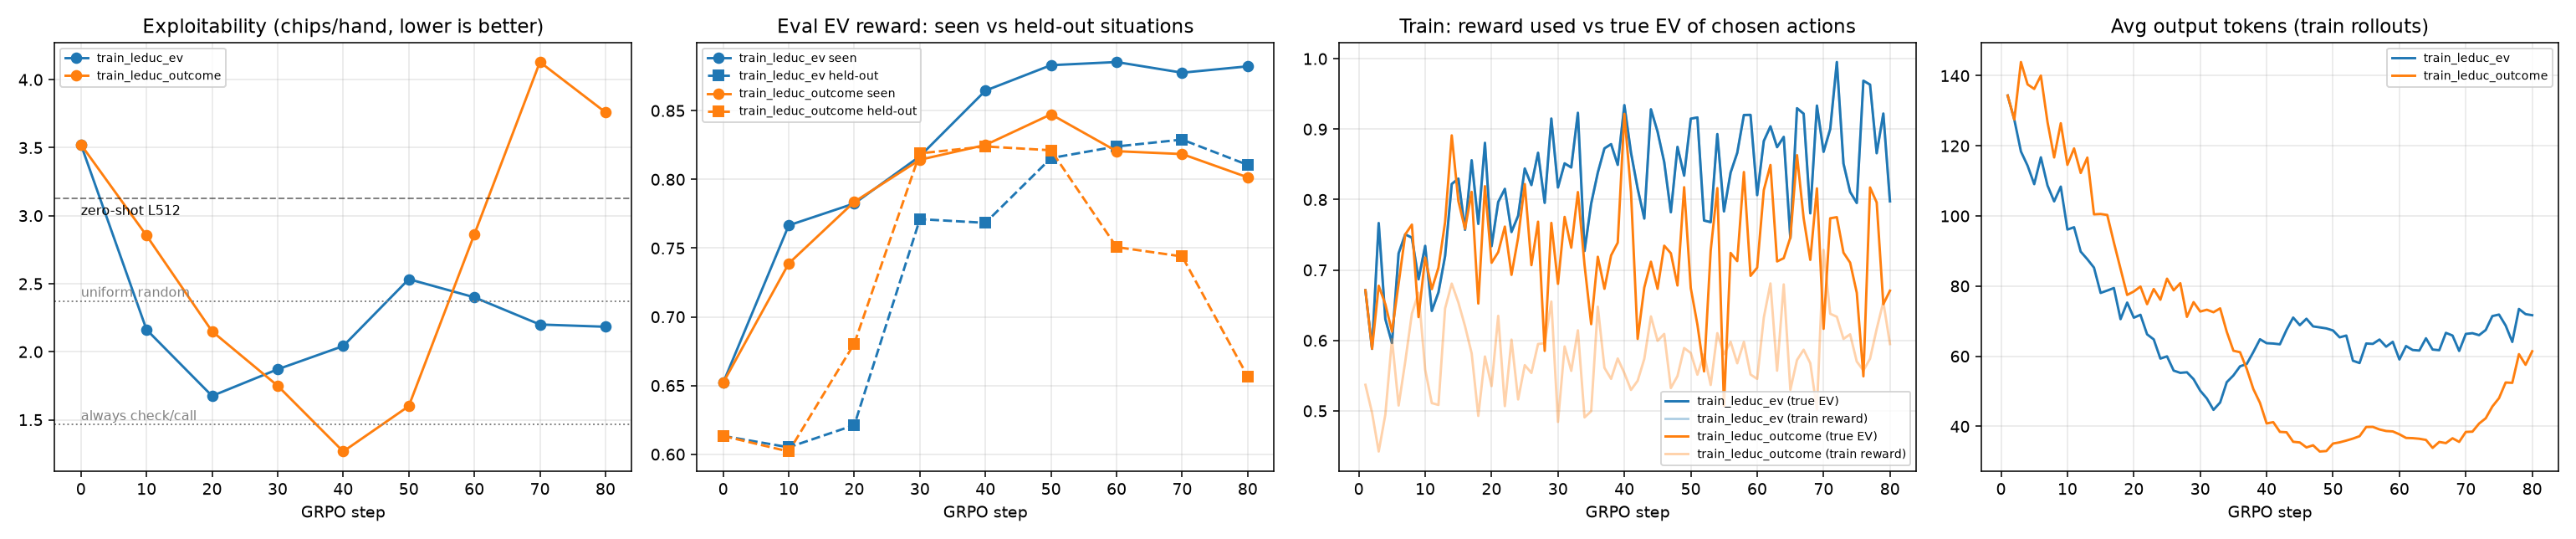
\includegraphics[width=\linewidth]{figures/p2_curves.png}
\caption{Training curves:
(1) exploitability;
(2) EV reward on seen (solid) vs held-out (dashed) situations;
(3) the training reward (faint) vs the true EV of the chosen actions;
(4) output length.
Evals before step 80 use $k=2$ and are noisy.}
\label{fig:p2}
\end{figure}

\section{Insights and difficulties}
\paragraph{Difficulty 1: no learning signal at first.}
\begin{itemize}
\item Our first full run used Qwen3's built-in thinking mode. The model wrote long analyses that often looped, and every
  rollout hit the 512-token limit.
\item So every reward was 0, all groups were identical, and the gradient was exactly 0. We stopped the run after 17 steps.
\item A prompt comparison fixed it:
\end{itemize}
\begin{center}\small
\begin{tabular}{lccc}
\toprule
Prompt & Valid answers & Hit the limit & Avg tokens\\
\midrule
Thinking mode, max 512 tokens & 0.04\% & 99.96\% & 512\\
Thinking off, same instruction & 45\% & 53\% & 326\\
\textbf{Thinking off + ``think briefly (a few sentences)''} & \textbf{95.8\%} & \textbf{0\%} & \textbf{140}\\
\bottomrule
\end{tabular}
\end{center}
\textbf{Insight:} with GRPO, the prompt must give the model a real chance of earning reward. The training script now stops
if fewer than 5\% of the step-0 answers are valid, so a run without signal cannot use up a GPU session.

\paragraph{Difficulty 2: the compute environment.} Kaggle's Python 3.13 is too new for vLLM, so we ran in a Python 3.12
environment. We also had to pin vLLM to the GPU it runs on: its Triton kernels crashed when run from the training GPU.

\paragraph{Insight: reward is not the objective.} The reward scores one decision against a fixed opponent. This turned out
to be the central issue in the analysis below.

\section{Analysis}
\paragraph{H1 holds with the exact reward.}
\begin{itemize}
\item Exploitability falls 30\% (3.13 $\to$ 2.18) and regret falls 81\%.
\item Held-out EV rises almost as much as seen EV (0.617 $\to$ 0.811 vs 0.652 $\to$ 0.882), although those situations
  were never trained on.
\item Example: facing a bet with a pair, the model now always calls, where zero-shot folded up to 60\% of the time.
\end{itemize}

\paragraph{H2 holds, more strongly than expected.}
\begin{itemize}
\item With the same compute, the noisy reward improves until about step 40 and then degrades.
\item It ends \emph{more} exploitable than zero-shot (3.76), and drifts into raising 89\% of the time (the equilibrium raises 39\%).
\item The reward it trains on stays flat at about 0.55--0.60 while the true value of its actions moves underneath
  (Fig.~\ref{fig:p2}, panel 3).
\item With 80 steps $\times$ 16 situations, the updates follow noise as much as signal.
\end{itemize}

\paragraph{H3 holds.}
\begin{itemize}
\item \textbf{The policy stops mixing.} In the \code{ev} run, entropy where the equilibrium mixes its actions collapses
  from 0.64 to 0.06, so the policy stops bluffing.
\item \textbf{Reward and quality come apart.} Exploitability is lowest at step 20 (1.68) and then rises to about 2.2,
  while the EV reward keeps climbing.
\item \textbf{The final policy is a \emph{calling station}.} It folds to 22\% of bets (equilibrium: 42\%) and bets or
  raises 27\% of the time (39\%).
  \begin{itemize}
  \item That scores well against the fixed opponent.
  \item An adversary beats it by betting strong hands, so it ends more exploitable than the always-call bot (1.47).
  \end{itemize}
\item \textbf{The learning signal runs out.} By the end, 75\% of groups get identical rewards.
\end{itemize}

\paragraph{Is the model's reasoning correct?} Each round-2 answer says whether the hand is ``strong'' or ``weak''. We
checked that claim against the hand's real strength: its chance of winning a showdown against a random unseen opponent
card, counted as strong if above 50\%.
\begin{table}[H]
\centering\small
\resizebox{\linewidth}{!}{%
\begin{tabular}{lccc}
\toprule
 & Zero-shot & GRPO \code{ev} & GRPO \code{outcome}\\
\midrule
Hand-strength claim correct & \textbf{77\%} & 66\% & 65\%\\
Strong hands without a pair (K on J/Q, Q on K; win 62\%) called ``strong'' & 66\% & 0.1\% & 0.4\%\\
Best action chosen, but stated reason wrong & 258 & 579 & 460\\
Invented poker terms (``flush'', ``Ace'', ``10'') in 2,304 answers & 139 & 23 & 7\\
Mentions opponent's likely hand / pot arithmetic & 91\% / 93\% & 68\% / 16\% & 27\% / 26\%\\
\bottomrule
\end{tabular}}
\caption{Correctness of the stated reasoning (round-2 answers containing a strength claim).}
\label{tab:reason}
\end{table}
\textbf{Mostly no: the actions improved, the stated reasons did not.}
\begin{itemize}
\item \textbf{The rule it learned:} ``pair = strong, anything else = weak'', backed by a meaningless comparison of the
  private card with the \emph{public} card. Example: ``Your private card is K, and the public card is J. You have a low
  card (K vs J), so you are likely vulnerable.'' In fact K is the best hand on a J board apart from a pair of J's.
\item \textbf{Why the actions are still good:} in round 2, an equilibrium opponent mostly bets with a pair, so ``fold
  without a pair when facing a bet'' is close to correct.
\item \textbf{What training removed:} the untrained model's confusion, such as ``you have a flush (Q-Q)'' (no flushes
  exist), ``QT'' (no 10s exist), or claiming both ``strong hand'' and ``weak hand'' in one answer.
\item \textbf{The net effect:} reasoning that is shorter (140 $\to$ about 60 tokens), more consistent and less
  hallucinated, but simplistic and often wrong.
\end{itemize}
\textbf{Lesson:} the reward scores only the final action, so RL shaped the action and left the explanation unchecked. A
natural next step is a process reward, for example extra credit for a correct hand-strength claim, which this setup can
compute exactly.

\paragraph{Limitations.}
\begin{itemize}
\item One seed per reward.
\item Evals before step 80 use $k=2$; only 80 training steps.
\item The held-out split covers only round-2 card pairs.
\item The opponent is always the equilibrium.
\item The reasoning check uses a keyword rule and ignores what the betting reveals about the opponent's card.
\end{itemize}

\paragraph{Next steps this setup supports.}
\begin{itemize}
\item \textbf{Self-play reward} (score against the model's current policy) to prevent H3's collapse.
\item \textbf{Distribution-matching reward} (reward a group's action frequencies for matching the equilibrium) to teach
  bluffing at the right rate.
\item \textbf{Variance reduction} for \code{outcome} (average several simulated hands), to measure how much of H2's gap it
  recovers.
\item \textbf{Process rewards} for correct intermediate claims.
\item \textbf{Full-hand, multi-turn RL}, with one reward per hand.
\end{itemize}
\end{document}
